% Drawing 23/05-1 -- folder 23, batch 05, archive page 91 (PDF page 92).
% Transcription: croquis à gauche, encre sur crayon : deux disques l'un au-dessus de l'autre, $X'$ en haut et $X''$ en bas ; dans chacun, des traits rayonnent d'un centre marqué, avec les lettres $Z'_0$, $Z'$ (en haut) et $Z''_0$, $Z''$ (en bas), et un trait épais sort du disque vers la gauche jusqu'à une légende ($V(f')$, $V(f'')$, lecture incertaine) ; à droite une grande courbe $D$ entoure les deux disques, et deux flèches partent de la région de $D$ vers l'intérieur de chaque disque ; le disque du bas est doublé d'un second contour marqué $X''$.
% Kind: two discs X' and X'' with rays from their centres, joined by a curve D. Method 2 (schematic redraw from the facsimile). Status: partial.
% Notes: The two discs (drawn as ellipses fitted to his outlines), each with its marked centre and the strokes radiating from it, all drawn from the one centre: in the upper disc six strokes, the upper left one heavy and running out of the disc to the legend at the left, the lower right one heavy; in the lower disc four strokes, the left one heavy and running out of the disc to a small heavy triangle of strokes at the left. The letters Z'_0, Z' and Z''_0, Z'' inside the discs and X', X'' beside them, where he wrote them. The large curve D, open at the top left and at the bottom left, passing at the right of both discs, with its letter. The two arrows from the region of D into the discs (to the upper disc from the right, to the lower disc from the upper right), and the short heavy stroke beside their tails. The second outline round the lower disc, from its upper left over the top to the right. Left out: the two legends at the far left (read V(f') and V(f'') with doubt; overwritten), a struck blot above the lower legend, the second « X'' » and the words of the text at the right of the crop. Still differs: free strokes read on a crowded sketch; the number of rays in each disc and the exact course of D are approximate. Redrawn 2026-11-12 (issue 128): to check again.
% Coordinates: 1 unit = 1 mm = 1/100 of the crop width (bbox in page fractions: [0.09, 0.2, 0.37, 0.45]).
% Redrawn by Claude (claude-fable-5-2), issue #128, 2026-11-12; not checked by a human; not compiled (no TeX in the session).
% Rights: reproduces part of the work -- behind RENDER_TRANSCRIPTS, never published by itself.
\documentclass[tikz,border=3pt]{standalone}
\usepackage{amsmath,amssymb}
\usetikzlibrary{patterns,arrows.meta}
\tikzset{pencil/.style={black!45}, struck/.style={black!35}, mpt/.style={circle,draw,inner sep=1.3pt}, pt/.style={circle,fill,inner sep=0.9pt}, opt/.style={circle,draw,fill=white,inner sep=1.1pt}}
\begin{document}
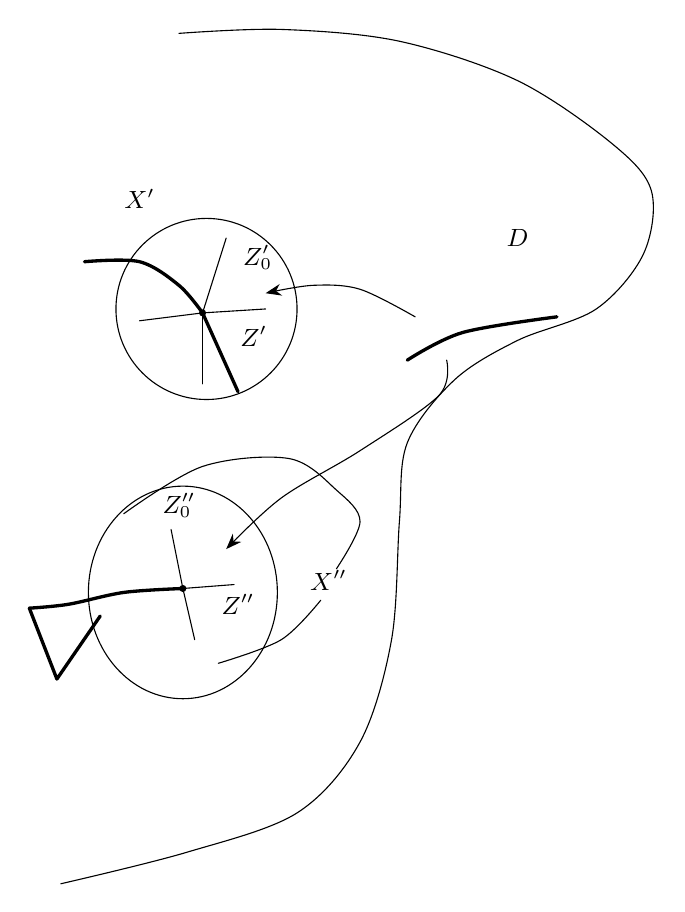
\begin{tikzpicture}[x=1mm,y=1mm,line cap=round,line join=round,font=\scriptsize]
\draw (30.5,-43) ellipse[x radius=11.5, y radius=11.5];
\node[pt] at (30,-43.5) {};
\draw[very thick] plot[smooth, tension=0.55] coordinates {(30,-43.5) (27,-40) (22,-37) (15,-37)};
\draw (30,-43.5) -- (33,-34);
\draw (30,-43.5) -- (38,-43);
\draw (30,-43.5) -- (22,-44.5);
\draw (30,-43.5) -- (30,-52.5);
\draw[very thick] (30,-43.5) -- (34.5,-53.5);
\node[inner sep=1pt] at (22,-29) {\small $X'$};
\node[inner sep=1pt] at (37,-36.5) {\small $Z'_0$};
\node[inner sep=1pt] at (36.5,-46.5) {\small $Z'$};
\draw[-{Stealth[length=2mm]}] plot[smooth, tension=0.55] coordinates {(57,-44) (50,-40.5) (44,-40) (38,-41)};
\draw plot[smooth, tension=0.55] coordinates {(27,-8) (40,-7.5) (55,-9) (70,-14) (82,-22) (87,-28) (86,-36) (80,-43) (70,-47) (62,-52) (56,-60) (55,-70) (54,-85) (50,-98) (42,-107) (28,-112) (12,-116)};
\node[inner sep=1pt] at (70,-34) {\small $D$};
\draw[very thick] plot[smooth, tension=0.55] coordinates {(56,-49.5) (63,-46) (75,-44)};
\draw[-{Stealth[length=2mm]}] plot[smooth, tension=0.55] coordinates {(61,-49.5) (60,-54) (50,-61) (40,-67) (33,-73.5)};
\draw (27.5,-79) ellipse[x radius=12, y radius=13.5];
\node[pt] at (27.5,-78.5) {};
\draw[very thick] plot[smooth, tension=0.55] coordinates {(27.5,-78.5) (20,-79) (13,-80.5) (8,-81)};
\draw[very thick] (8,-81) -- (11.5,-90) -- (17,-82);
\draw (27.5,-78.5) -- (26,-71);
\draw (27.5,-78.5) -- (34,-78);
\draw (27.5,-78.5) -- (29,-85);
\draw plot[smooth, tension=0.55] coordinates {(20,-69) (30,-63) (41,-62) (47,-66) (50,-70) (47,-76)};
\draw plot[smooth, tension=0.55] coordinates {(45,-80) (40,-85) (32,-88)};
\node[inner sep=1pt] at (27,-68) {\small $Z''_0$};
\node[inner sep=1pt] at (34.5,-80.5) {\small $Z''$};
\node[inner sep=1pt] at (46,-77.5) {\small $X''$};
\end{tikzpicture}
\end{document}
